\documentclass[a4paper, 12pt]{scrartcl}

\usepackage{scrpage2}
\usepackage[left=2.5cm,right=2.5cm, top=3cm, bottom=4cm]{geometry}
\usepackage[utf8]{inputenc}
\usepackage[ngerman]{babel}
\usepackage[T1]{fontenc}
\usepackage{amsmath}
\usepackage{amssymb}
\usepackage{amsfonts}

\usepackage{graphicx}

\usepackage{float}
\usepackage{adjustbox}
\usepackage{hyperref}
\usepackage{textcomp}
\usepackage{multirow}
\usepackage{array}

%\usepackage{enumerate}
\usepackage[shortlabels]{enumitem}

% Einrücken verhindern
\setlength{\parindent}{0em} 


\begin{document}

\begin{titlepage}
	\centering
	{\Huge\bfseries Versuchsprotokoll\par}
	\vspace{2cm}
	{\scshape\LARGE Wärmelehre \par}
	\vspace{1cm}
	{\Large Bestimmung des Adiabatenkoeffizients \\ mit der Rüchardt-Methode\par}
	\vfill
	{\large\itshape Simon Schwarz und Marius Ising\par}

	\vfill
\end{titlepage}

\tableofcontents
\newpage

\section{Rüchardt-Methode}

Wir wollen den Adiabatenkoeffizient $\kappa = \frac{c_p}{c_v}$ von Luft mit der Rüchardt-Methode bestimmen. Dabei ist $c_p$ die spezifische Wärme bei konstantem Druck und $c_v$ die spezifische Wärme bei konstantem Volumen. Die Rüchardt-Methode beruht auf der Messung von Schwingungen einer Stahlkugel.

\begin{figure}[H]
\centering
\includegraphics[width=.5\textwidth]{bilder/prinzipRuechardt.jpg}
\caption{Prinzip der Messung von $\kappa$ nach Rüchardt}
\end{figure}

Die Kugel befindet sich im Gleichgewicht, wenn der Druck $p$ in der Flasche gleich der Summe aus dem Außendruck $p_0$ und dem Druck der Gewichtskraft der Kugel ist. Dann gilt
$$p = p_0 + \frac{mg}{A}$$
mit der Querschnittsfläche $A = \pi \frac{D^2}4$ des Glasrohrs. Lenkt man die Kugel um eine Strecke $x$ aus der Gleichgewichtslage aus, so ändert sich der Druck um $dp$ und es wirkt eine Kraft $A dp$ auf die Kugel. Mit der Reibungskraft $F_R = \alpha \frac{dx}{dt}$ ergibt sich dann
$$m \frac{d^2x}{dt^2} = Adp - \alpha\frac{dx}{dt}.$$
Der Prozess wird als quasi adiabatisch betrachtet, da er für einen Wärmeaustausch zu schnell abläuft. Damit gilt die Differenzialgleichung der Adiabate
$$\frac{dp}{p} = - \kappa \frac{dV}V.$$
Mit der Volumenänderung $dV = Ax$ erhält man die Bewegungsgleichung
$$\frac{d^2x}{dt^2} + \frac{\alpha}m \frac{dx}{dt} + \frac{p\kappa A^2}{mV}x = 0.$$
Dies ist die Differenzialgleichung einer gedämpften harmonischen Schwingung. Aus der Schwingungsfrequenz $\omega_0^2 = \frac{p\kappa A^2}{mV}$ der ungedämpften Schwingung ergibt sich dann
$$\kappa = \omega_0^2 \frac{mV}{pA^2}.$$
Mit dem Dämpfungsfaktor $\delta = \frac{\alpha}{2m}$ und der Schwingungsfrequenz $\omega$ der gedämpften Schwingung erhält man
$$\omega_0^2 = \omega^2 + \delta^2.$$



\section{Versuchsaufbau}



\begin{figure}[h]
\centering
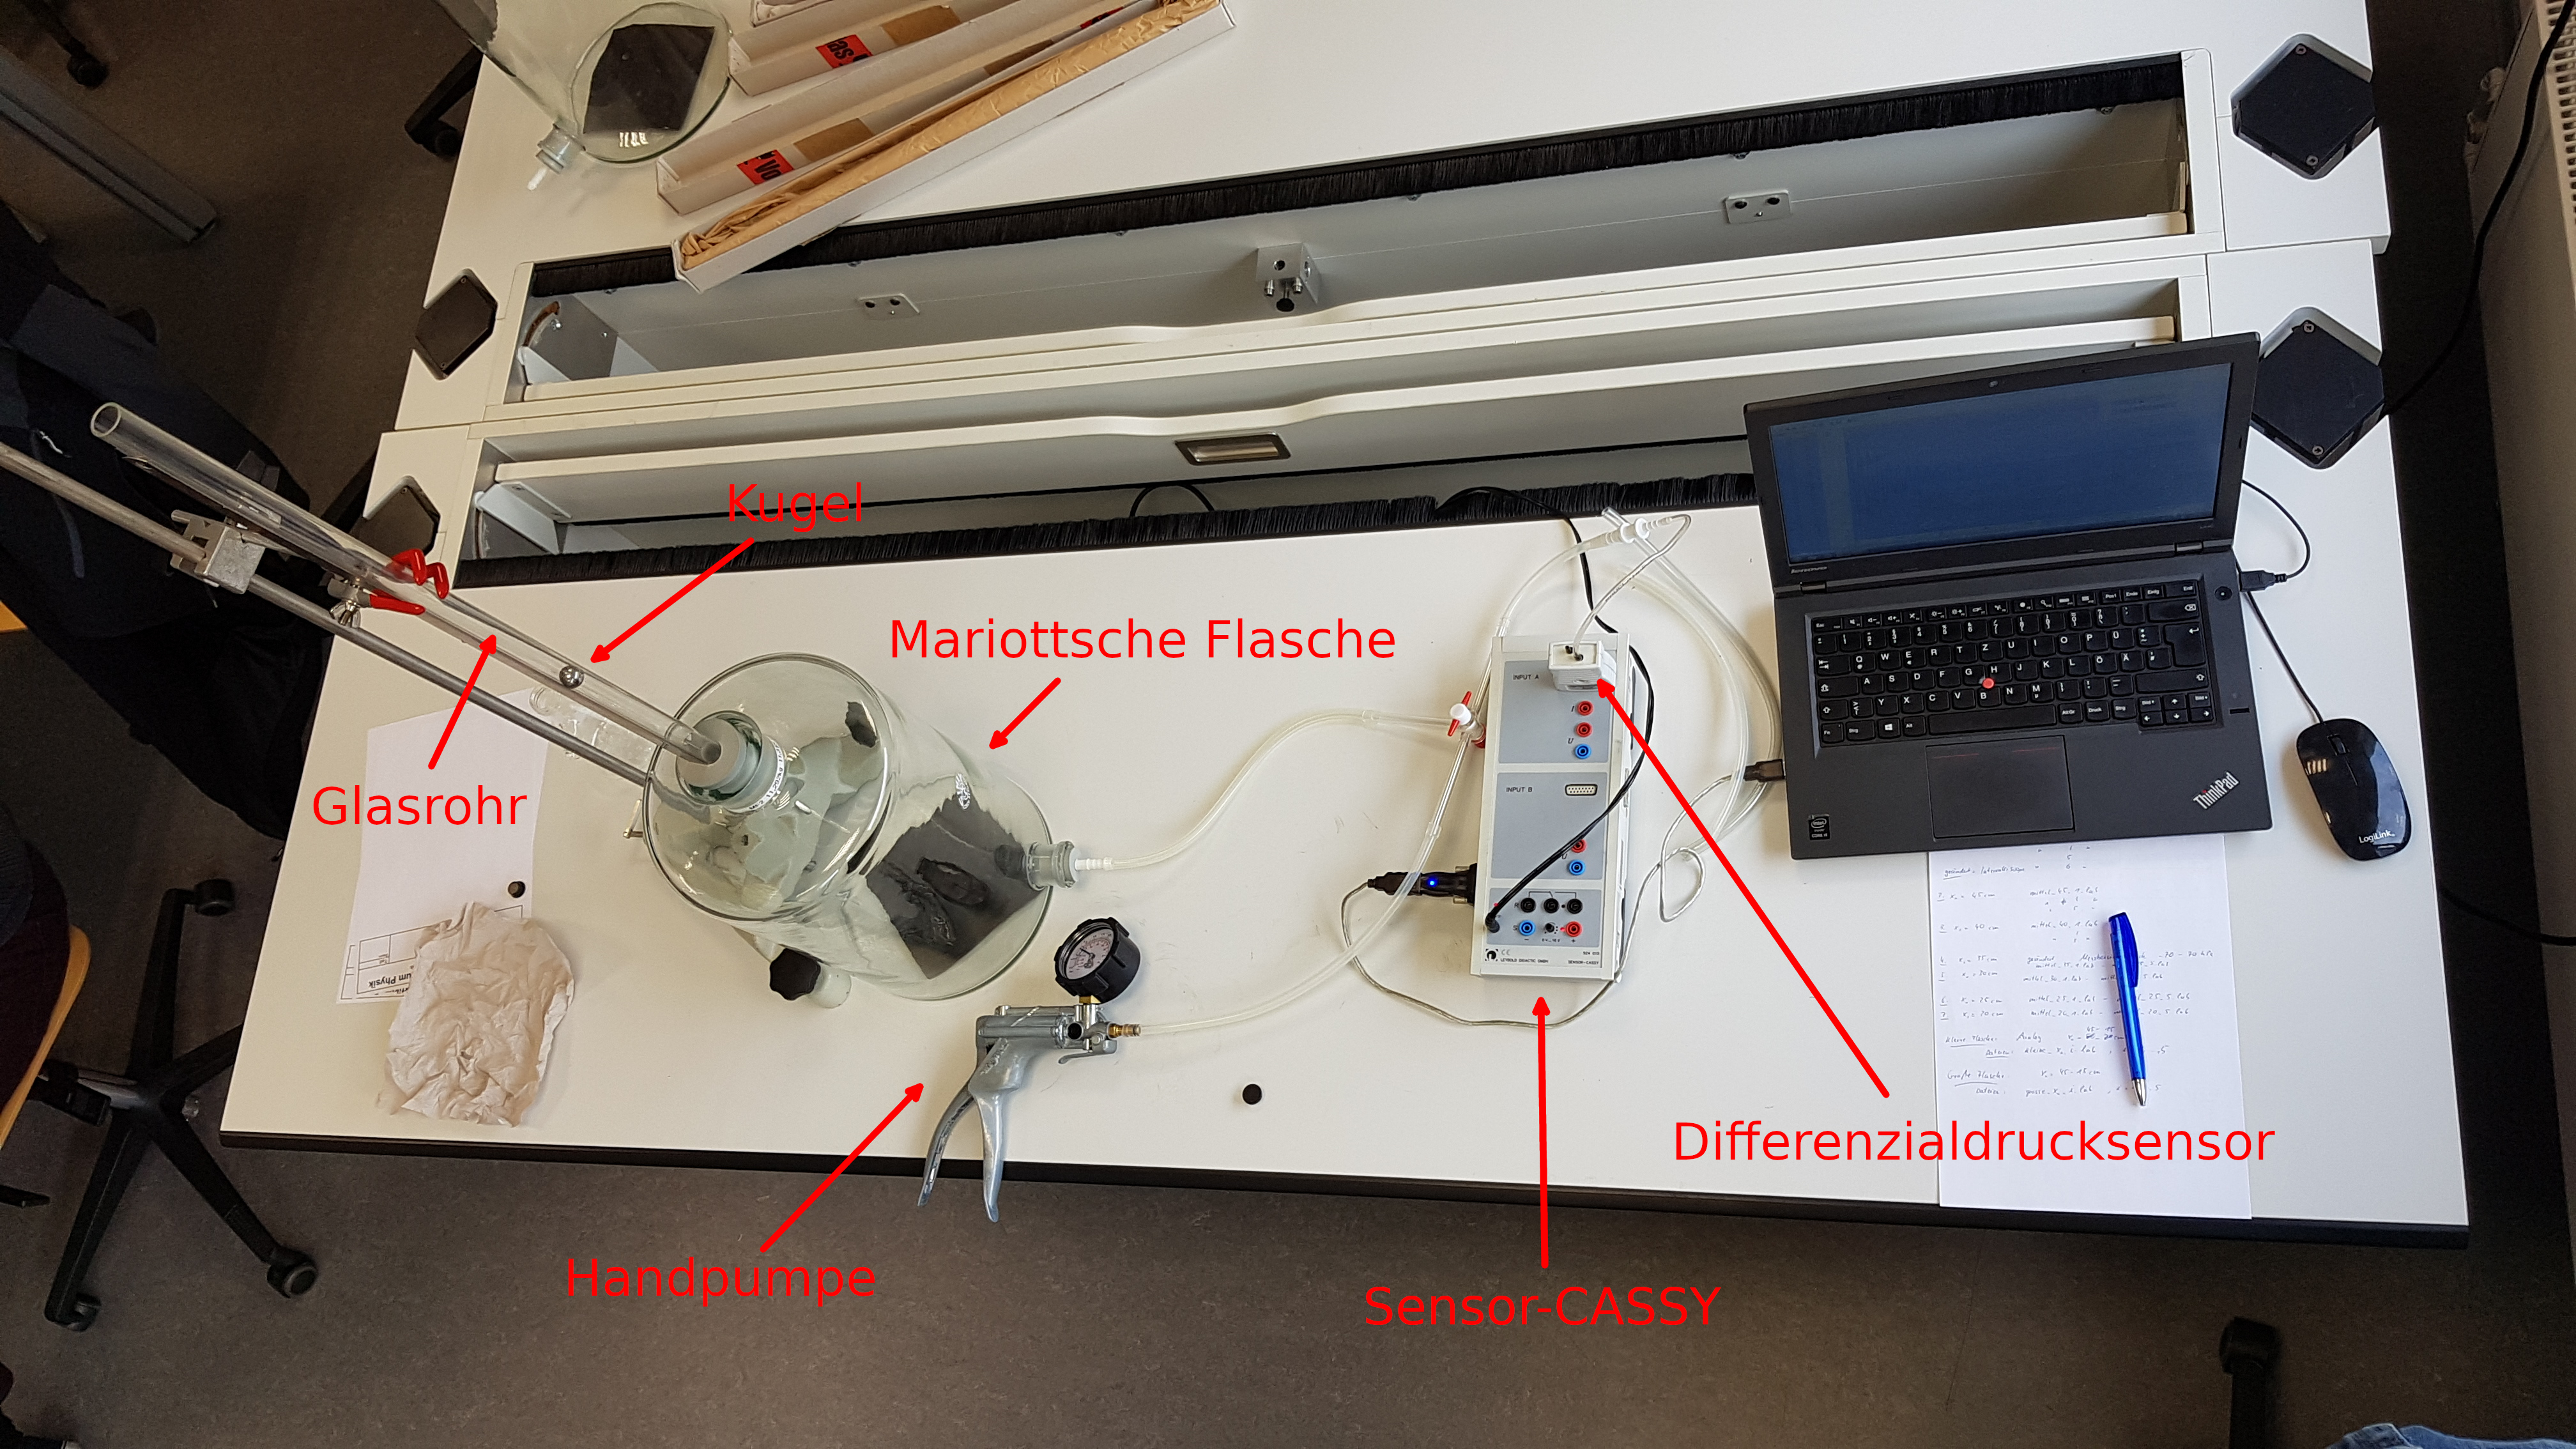
\includegraphics[width=\textwidth]{bilder/aufbau_beschriftet.jpg}
\caption{Versuchsaufbau}
\end{figure}
In die Mariottsche Flasche wird vertikal ein Glasrohr eingeführt, welches durch einen Gummiring luftdicht abgeschlossen ist. Die vertikale Position das Rohrs wird mit einer Greifhalterung, die an einem Stativ befestigt ist, fixiert. Zusätzlich wird an die Halterung ein Metallmaßstab angebracht. In den Auslass der Mariottschen Flasche wird über ein Schlauch und eine T-Ventil eine Handpumpe und ein Differenzialdrucksensor angeschlossen. Der Sensor wird dabei an den Eingang A des Sensor-CASSY angeschlossen. Es stehen insgesamt drei Flaschen mit unterschiedlichen Größen zur Verfügung.



\section{Versuchsdurchführung}

Die Masse $m$ der Kugel wird mittels einer Digitalwaage und der Durchmesser $D$ mit einer Mikrometerschraube gemesssen. Der Außendruck $p_0$ wird von einer Wetterstation am Campus Hörn abgerufen. Der Versuchsaufbau wird nacheinander mit den drei Mariottschen Flaschen aufgebaut. Für jede Flasche wird die Schwingung bei 6-7 verschiedenen Starthöhen $x_0$ aufgezeichnet. Die Starthöhen werden zwischen $50 \, \mathrm{cm}$ und $15 \, \mathrm{cm}$ gewählt und in Schritten von $5 \, \mathrm{cm}$ geändert. Dabei werden für jede Höhe 5 Messungen des Differenzialdrucksensors aufgezeichnet. Für den Relativdruck wird zwischen dem Messbereich von $\pm 21 \, \mathrm{hPa}$ und $\pm 70 \, \mathrm{hPa}$ variiert. Für die Messung mit dem Sensor-CASSY werden folgende weitere Messparameter gewählt:
\begin{enumerate}[-]
\setlength{\itemsep}{-5pt} 
\item Intervall: $500\,\mu$s 
\item Messungen: $16000$
\item Messzeit: $8\,$s
\end{enumerate}
Für die Höhe $x_0 = 50 \, \mathrm{cm}$ bei der mittleren Flasche ist das Messintervall abweichend auf $200 \,\mu\mathrm s$ festgesetzt. Zusätzlich wurde bei dieser Höhe noch eine Messung mit den anderen Parametern durchgeführt. Das Volumen der kleinen und der mittleren Flasche wird mittels Wiegung der leeren und der mit Wasser gefüllten Flasche nach dem eigentlichen Versuch bestimmt. Für das Volumen der großen Flasche wird der auf einem Aufkleber angegebene Wert benutzt. 



\section{Versuchsauswertung}

\section{Fazit}

\end{document}
